\subsubsection{Asynchronous Processing Pipeline}

The asynchronous flow is hosted in an Azure Function. The \texttt{[ServiceBusTrigger]} attribute establishes the connection between the Azure Service Bus queue and the function's \texttt{ProcessExpenseFromQueue} implementation. This attribute instructs Azure Functions to execute the \texttt{Run} method whenever a new message appears in the queue named \texttt{expense-processing-queue}. This process is illustrated in Figure~\ref{fig:servicebus-trigger}.

\begin{figure}[H]
    \centering
    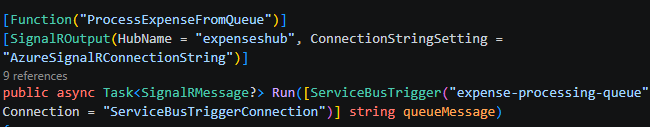
\includegraphics[width=0.8\textwidth]{Images/Implementation/ProcessExpenseFromQueue.png}
    \caption[Run method implementation in ProcessExpenseFromQueue.cs]
    {\texttt{Run} method implementation in \texttt{ProcessExpenseFromQueue.cs}. [Own creation]}
    \label{fig:servicebus-trigger}
\end{figure}